\chapter{Implementation of Privacy Protection Measures}
\section{Privacy Policy}

In complience legal requirements of the Data Protection Directive (cf. Section \ref{EUDIR}) we include the following
Privacy Policy on our Mobile Application and Website.

\begin{quote}
\tt \small
\textbf{Privacy Policy}\\
==============

\textbf{What Personal Information do we Collect?}\\
The Mobile Sensor Collection Application collects the following data from your mobile phone:\\
- Sensor Data from Accelerometer (50Hz)\\
- Sensor Data from GPS sensors (~every 30 sec)\\
- Daily Human Activities (walking, standing, sitting, etc.) (every 30sec)\\
- Used Service Lines (bus, train, tram) (every 2 minutes)\\

All collected data is transferred to our data center.

The Live+Gov Services does NOT store or collect names and email addresses.

\textbf{Which processing is applied to the data?}\\
We process Accelerometer samples on the Mobile device in order to extract human activities.
We process GPS coordinates on the Live+Gov server to extract the currently used service lines.

The stored information is used to produce aggregate reports.
These reports are based on anonymized data that do not allow the reconstruction of the routes of individual persons at a given point in time.

\textbf{When is the data deleted?}\\
The full data-set will be stored until January 2015.

Afterwards we will delete Names and Email addresses and anonymize
the sensor data and processing results.  The anonymized data will
be used by the the Consortium Partners for research purposes.

\textbf{For which purposes is the data collected?}\\
The collected data will be used for personalization of user experience of the mobile application.
Moreover, we will analyize travel patterns in the Helsinki Urban region for general research and for improvement and optimization of the
infrastructure provided by HSL.

\textbf{Identity of Data Controller}\\
The data is controlled by Heinrich Hartmann <hartmann@uni-koblenz.de>

The following organizations have access to the collected data:
\begin{enumerate}
\item University of Koblenz-Landau
\url{http://www.uni-koblenz-landau.de/}\\
Universitätsstraße 1\\
56070 Koblenz

\item Mattersoft
\url{http://www.mattersoft.fi/}
Hämeenkatu 13, 33100 Tampere, Finland\\
+358 10 3225000

\item Centre for Research and Technology Hellas (CERTH)
\url{http://mklab.iti.gr/contact}\\
6th km Charilaou-Thermi Road\\
P.O. Box 60361,\\
57001 Thermi-Thessaloniki, Greece
\end{enumerate}

\textbf{Access to Stored Data}\\
All personal data can be accessed at our Privacy Dashboard at
\url{http://liveandgov.uni-koblenz.de/trial/dashboard}

There you have the possibility to:\\
- View all recordings made\\
- View the raw data collected for each recording\\
- Download the data for each recording\\
- Delete records

\textbf{Collaboration with Third Parties}\\
The raw data is not shared with any parties external to the Live+Gov Consortium.

Aggregated report based on anonymized data are disclosed to officials at HSL \url{http://www.hsl.fi/} and might be made
public in the form of a blog post or research article.  These aggregated reports show distributions of all routes that
have been collected in the system and do not allow to infere the location of a single user at a given point in time.

\textbf{Consent}\\
I have read and understood the above privacy policy and agree that my data is collected and processed accordingly.
\end{quote}

\section{Privacy Dashboard}
The Live+Gov Privacy Dashboard is a software component that allows the
citizens to view the data about themselves that is stored in the
Sensor Data Storage server.  The foundation of the Privacy Dashboard
component is the inspection tool that was introduced in D1.1 as a
means to perform basic quality controlling of the collected data.

The Privacy Dashboard is currently endowed with the following views:
\begin{itemize}
  \item \textbf{Login Screen} (cf. Figure \ref{fig:PDLogin}).  Before
    access to the dashboard is granted, the user is prompted for
    credentials.  The credentials are generated by the sensor
    collection application on the mobile device.  The username can be
    freely chosen by the user. The password is then generated by the
    mobile application and transferred to the server alongside with
    the recording.
 \item \textbf{Recording Overview.} (Cf. Figure \ref{fig:PDOverview}).
   This view shows all recordings that the user submitted to the Data
   Storage Service including basic meta information like start data of
   recording, duration. The user can click on each recording in order
   to view the recorded data in the Raw Data View.

   An important feature of the recording overview table is the delete
   button (cross on the very left.) That allows the user to
   selectively delete recordings, that shall not be analyzed by the
   Live+Gov system. Internally the click on the delete button only
   flags the corresponding trip for deletion. The actual deletion is
   carried out as a batch job on a regular bases. This addition step
   prevents accidental loss of data.

 \item \textbf{Raw Data View.} (cf. Figure \ref{fig:PDRawData}) The
   raw data view shows all recorded raw data to the user.  GPS data is
   visualized on a map. Motion sensor data is displayed as plots. Wifi
   and GSM data is displayed in lists.
   The raw data from each sensor can be downloaded individually as CSV file.

 \item \textbf{Processing View.} (cf. Figure
   \ref{fig:PDProcessedData}).  The processing view shows the data
   mining end-products for each processing step.  The Figure shows the
   processing view for the Activity Recognition. On the top a
   time-line is show that visualizes the different recognized
   activities via color-coding. A map below displays the corresponding
   GPS track with the same color coding.

   A similar view for Service Line Detection results is currently
   under development.
\end{itemize}

\begin{figure}
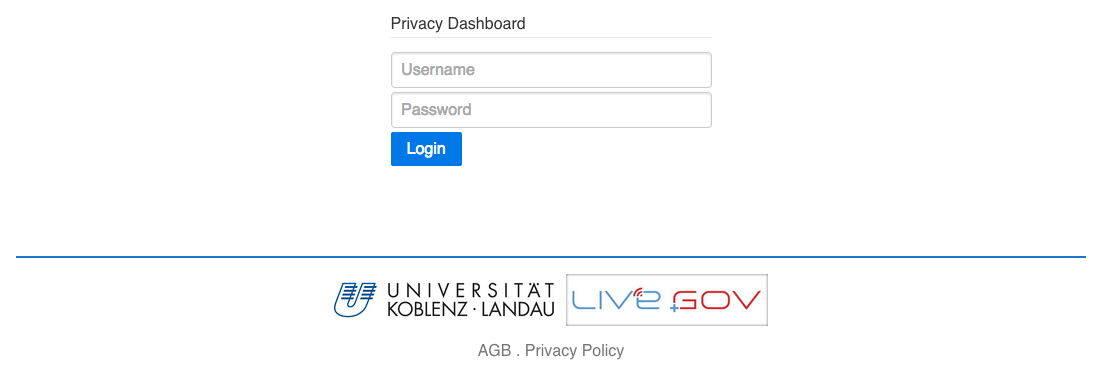
\includegraphics[width=\textwidth]{screenshots/login.png}
\caption{Live+Gov Privacy Dashboard Login}
\label{fig:PDLogin}
\end{figure}

\begin{figure}
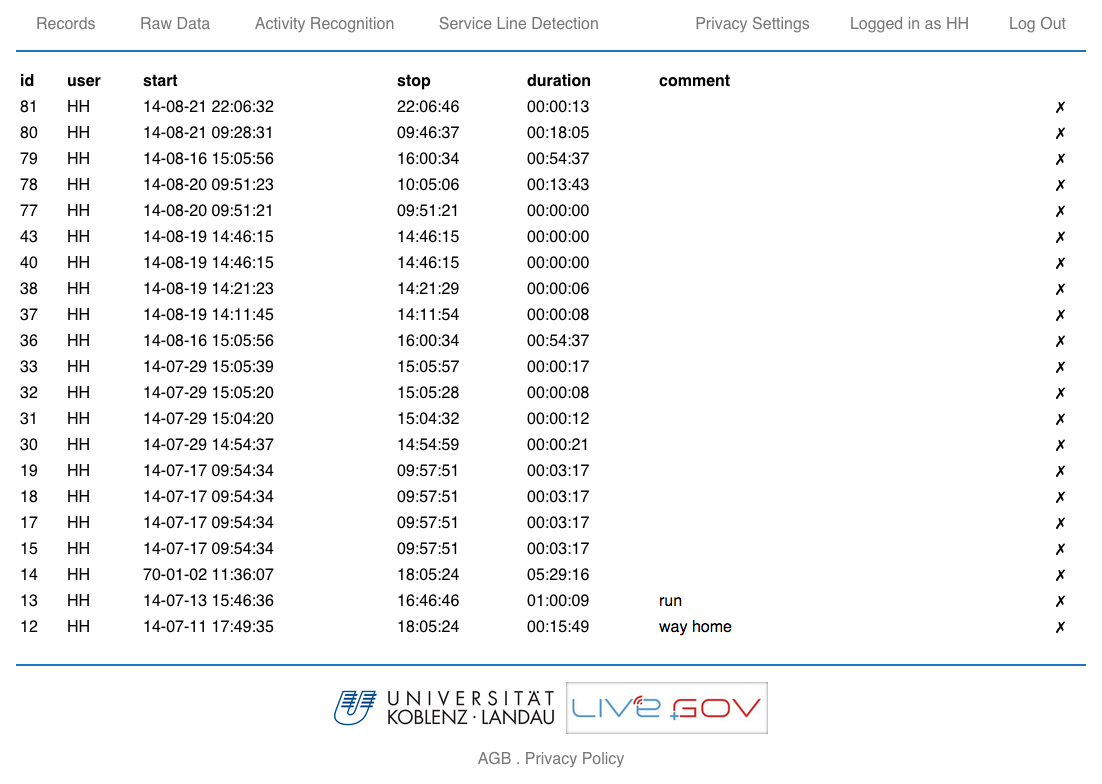
\includegraphics[width=\textwidth]{screenshots/recordings.png}
\caption{Live+Gov Privacy Dashboard Recording Overview}
\label{fig:PDOverview}
\end{figure}

\begin{figure}
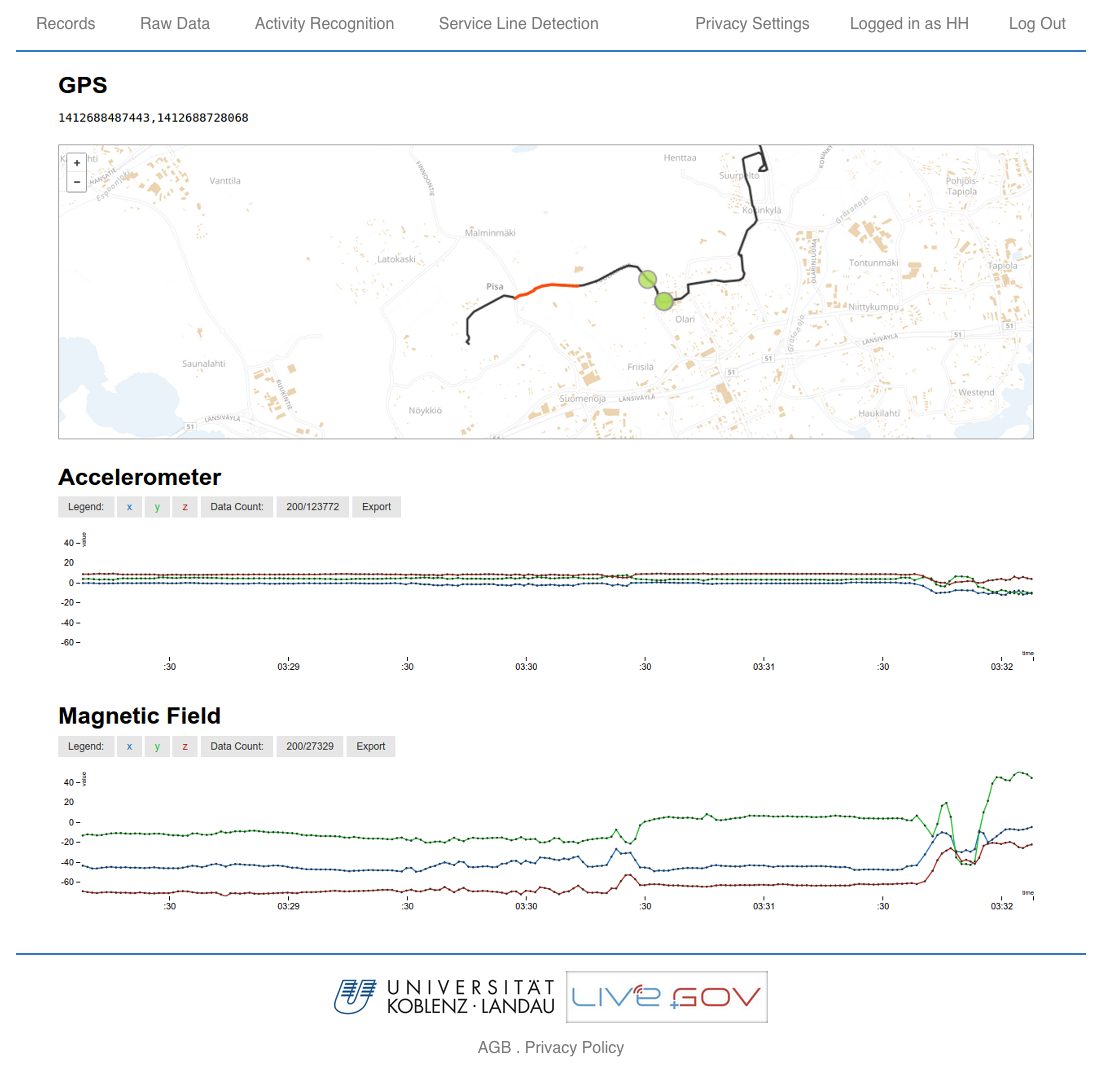
\includegraphics[width=\textwidth]{screenshots/raw.png}
\caption{Live+Gov Privacy Dashboard Raw Data View}
\label{fig:PDRawData}
\end{figure}

\begin{figure}
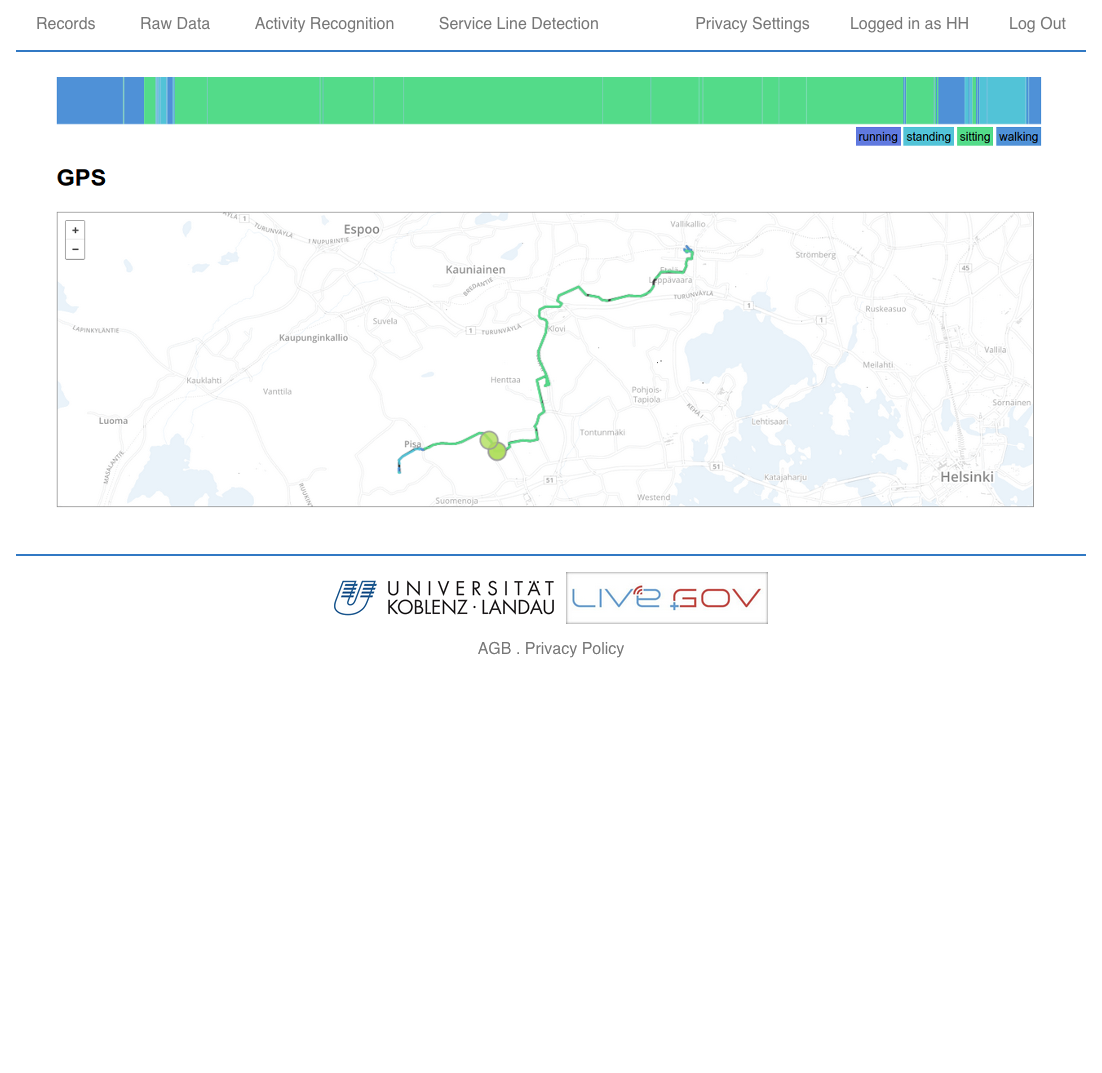
\includegraphics[width=\textwidth]{screenshots/processed.png}
\caption{Live+Gov Privacy Dashboard Processed Data View}
\label{fig:PDProcessedData}
\end{figure}

\section{Transfer Encryption (HTTPS/SSL)}
The data transfer from the mobile device to the Data Storage component
as well as the transfer to the Privacy Dashboard relay on HTTP. In
order to avoid eavesdropping by externals that have access to the
communication channels, we secured all HTTP connections with SSL
encryption.

The implementation of this measure was rather straight forward. A SSL
certificate was issued by the University of Koblenz, and installed to
our webservers. Requests to this servers can now be done using HTTPS.
Figure \ref{fig:PDHTTPS} shows a screenshot of such a secured
connection to our Privacy Dashboard. The necessary adjustments to the
Sensor Collection Component were minimal, since Android comes with
native support for HTTPS connections.

\begin{figure}[h]
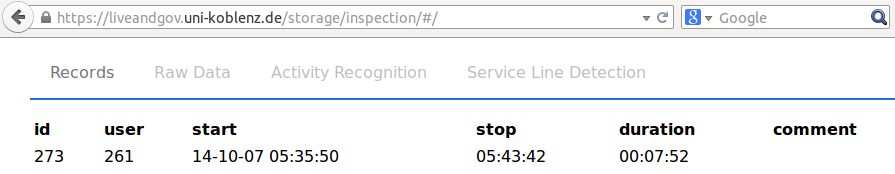
\includegraphics[width=\textwidth]{screenshots/HTTPS.png}
\caption{HTTPS connection to Privacy Dashboard}
\label{fig:PDHTTPS}
\end{figure}

\section{Data Expiring Dates}
Trips stored in the Sensor Data Storage Service have been endowed with
a data expiration date. A python script is provided that performs the
of expired data. In our installation we have this script running as a
cron job every night. The resulting schema of the trip table listed in
Figure \ref{fig:TripScheme}.

By default the expiration data is set to one year after the recording
was uploaded. We are working on including a feature for setting the
expiration date for each recording inside the privacy dashboard.

\begin{figure}
\centering
\begin{verbatim}
  Column  |          Type
----------+------------------------
 trip_id  | integer
 user_id  | character varying(36)
 start_ts | bigint
 stop_ts  | bigint
 name     | character varying(255)
 deleted  | boolean
 expires  | bigint
\end{verbatim}
\caption{Database Schema of the Trip Table}
\label{fig:TripScheme}
\end{figure}

\section{Anonymization of trips}
The Sensor Data Storage Service follows a privacy by design guideline
in that it does not store personal information like names and email
address at all.

In the case that such information should be linked to the user-id
stored in the trip table we provide a python script that randomizes
the user-ids and thereby removes all links that might have existed
before.

\begin{figure}[fontsize=\tiny]
\centering
\begin{verbatim}
Usage: privacy.py [-d database name] [-u database user]
                  [-p database password]
                  [-h database host] [-o operation]

Valid Operations:

cleanup: Flags all expired rows as deleted
    No Options

anonymization: Sets all user_ids to 0
    Option:
        SQL Select Query: Every row found by this query will
        be set to user_id = 0.

haircut: Cuts trips where they split and could be traceable
    Options:
        First - the radius in which we look
        Second - the number of users that needs to be in the
                 radius

blur: Offsets every GPS point by a random amount
    Options:
        The maximum distance a point can have to its origin

k_anonymity: Creates a centroid for every GPS point
    Options:
        First - Number of maximum GPS points to use. If 0 then
                we grab every point inside the radius
        Second - Maximum distance a point can have to be used
                for the creation of the new point
\end{verbatim}
\caption{Usage options for the privacy.py script.}
\end{figure}

\section{K-Anonymity of GPS routes}
Python script that deletes all parts of journeys that have are not
near to at least k other journeys.

TODO: Insert Literature Reference.
TODO: Add screenshots.

\section{Randomization of GPS data}
Python Script that adds random noise to GPS data.
